\newpage
\section{Durchführung}
\label{sec:Durchführung}

\subsection{Versuchsaufbau}
\label{sec:Aufbau}

\begin{figure}
  \centering
  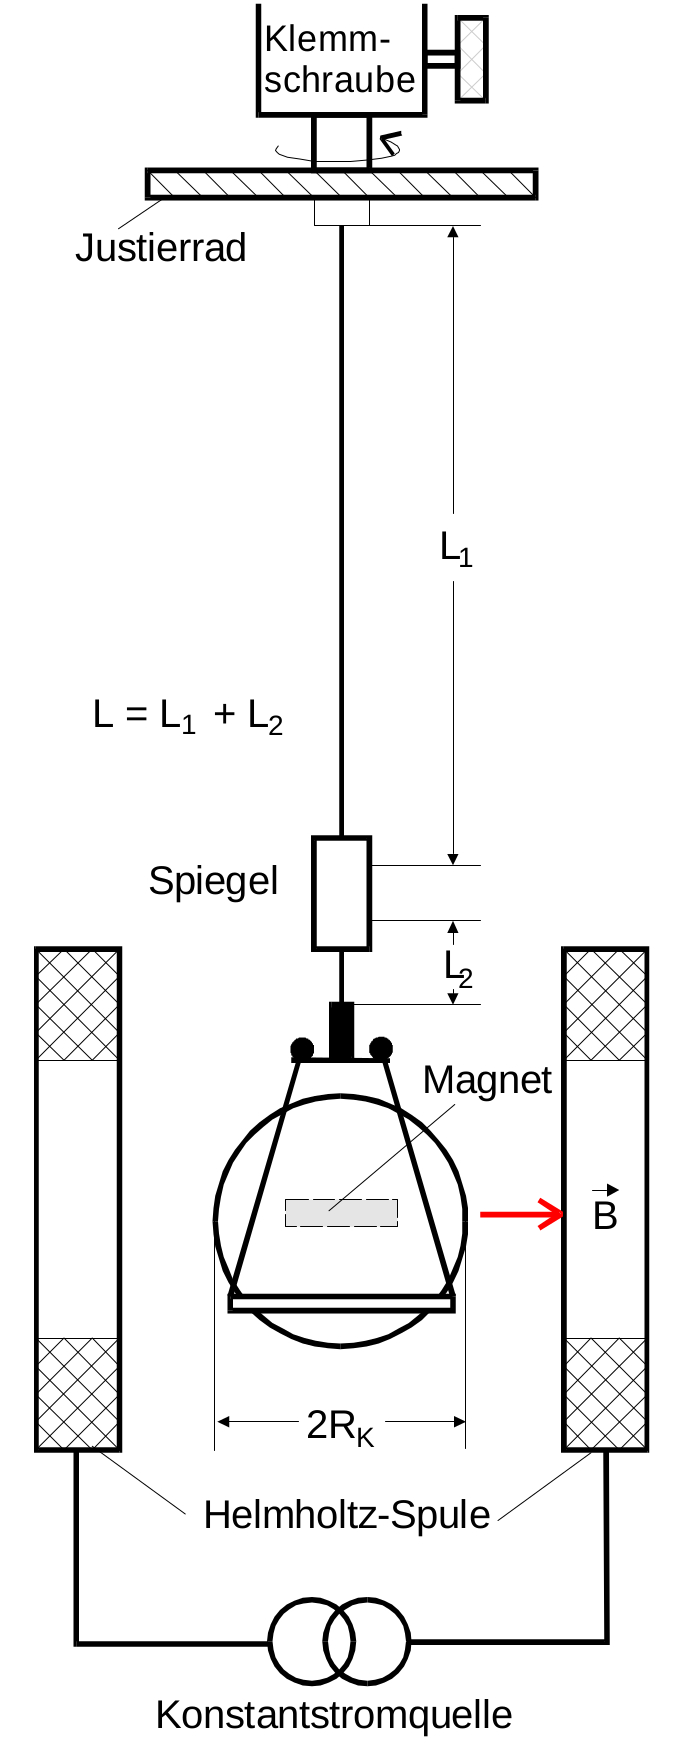
\includegraphics[height=7.0cm]{content/Versuchsaufbau.jpg}
  \caption{Skizze des verwendeten Versuchsaubaus  \cite{anleitung}.}
  \label{fig:Versuchsaufbau1}
\end{figure}

Eine Kugel ist an einem Torsionsdraht der Länge $L$ in einem Helmholtzspulenpaar
aufgehangen. Der Draht ist mit einem Spiegel versehen und kann mit
Hillfe eines Justierrades
tordiert werden, damit das System schwingt.
In der Kugel befindet sich ein kleiner Stabmagnet.
Die Periodendauer des
schwingenden Systems wird mit Hilfe
des in Abbildung \ref{fig:Versuchsaufbau2} dargestellten Aufbaus gemessen.
Bei der Durchführung ist darauf zu achten, dass ein Pendeln der Kugel zu
unterbinden ist.

\begin{figure}
  \centering
  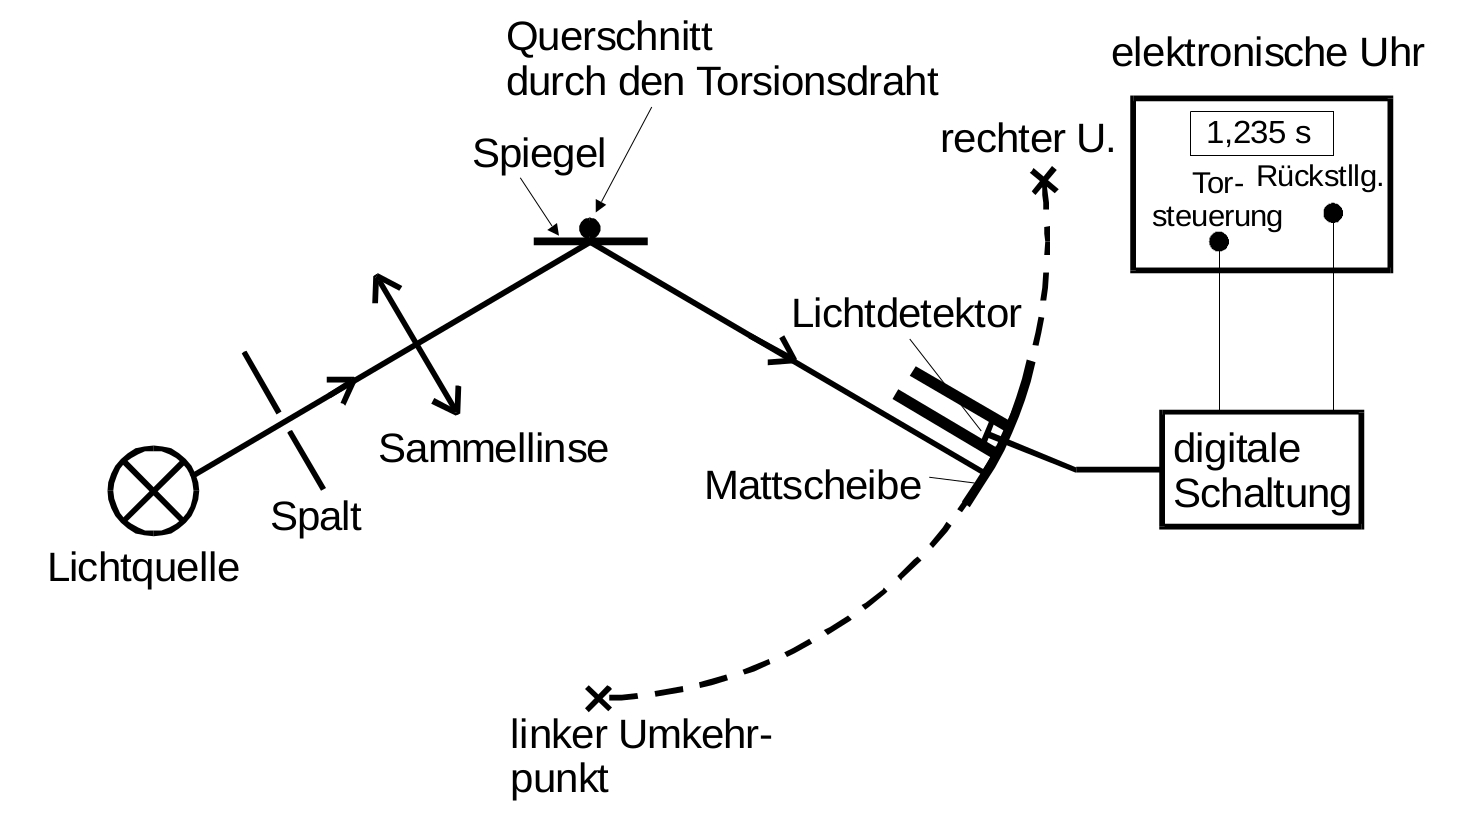
\includegraphics[height=7.0cm]{content/Spiegelanlage.jpg}
  \caption{Skizze des Aufbaus zur Messung der Periodendauer \cite{anleitung}.}
  \label{fig:Versuchsaufbau2}
\end{figure}

Ein von der Lichtquelle ausgehender Lichtstrahl wird gebündelt und am Spiegel
des Drahtes reflektiert. Diese Reflexion fällt bei einem bestimmten Winkel des
Spiegels in einen Lichtdetektor, welcher ein elektronische Zählwerk bedient. Die
Schaltung zwischen dem Lichtdetektor und der elektronischen Uhr, die aus zwei
auf die abfallende Flanke getakteten T-Flipflops und einer monostabilen Kippstufe besteht,
ist in Abbildung \ref{fig:Versuchsaufbau3} dargestellt.

\begin{figure}
  \centering
  
\includegraphics[width=\textwidth]{content/Schaltplan.jpg}
  \caption{Schaltplan zur Bedienung der elektronischen Uhr.}
  \label{fig:Versuchsaufbau3}
\end{figure}

Der erste Lichtimpuls startet die elektronische Uhr, der zweite wird nicht
benötigt und der dritte Lichtimpuls stoppt die Uhr, sodass auf ihr die
Periodendauer abzulesen ist. Der vierte Impuls setzt die Uhr zurück.

\subsection{Messung des Schubmoduls eines Drahtes}
\label{sec:elKonstanten}

Die Konstantstromquelle des Spulenpaares wird ausgeschaltet und das System mit
Hilfe des Justierrades ausgelenkt. Dabei ist darauf zu achten, dass die Auslenkung
mindestens so groß ist, dass der reflektierte Lichtstrahl den Lichtdetektor
erreicht und maximal so groß ist, dass die Kugel um bis zu \SI{360}{\degree}
schwingt. Die Kugel
wird in ihrer Aufhängung so gedreht, dass der Stabmagnet in Ruhelage
vertikal ausgerichtet ist.
Die auf der Uhr angezeigte Periodendauer wird für 12 Schwingungen gemessen.

\subsection{Messung des magnetischen Moments eines Magneten}
\label{sec:magMoment}

Der Strom der Konstantstromquelle wird zwischen
\SIrange[range-phrase = \:und\:]{0.1}{1.0}{\ampere} in
\SI{0.1}{\ampere}-Schritten variiert und für jede Einstellung werden fünf
Periodendauern gemessen. Vorher ist die Kugel in Ruhelage so zu drehen, dass der Stabmagnet
an dem Magnetfeld in Nord-Richtung des Helmholtz-Spulenpaares ausgerichtet ist.
Bei der Durchführung ist zu darauf achten, dass nur um kleine Winkel ausgelenkt werden
darf, damit die in Kapitel \ref{sec:magTheorie} beschriebene Kleinwinkelnäherung gilt.

\subsection{Messung der Horizontalkomponente des Erdmagnetfeldes}
\label{sec:Erdmagnetfeld}

Die Konstantstromquelle wird für diesen Versuchsteil ausgeschaltet.
Der Stabmagnet der Kugel wird in Ruhelage in Nord-Süd-Richtung ausgerichtet und
die Periodendauer wird für 12 Schwingungen gemessen.
